
\chapter{Conclusions and future work}

\textit{This is an except from my transfer report.}

\section{Introduction}

This chapter reviews my proposed methods for the estimation of vital signs using data recorded from wearable devices and video cameras. I also present future areas of research. During the first year of my DPhil, I developed signal processing algorithms to assess the quality of the information recorded by the Wavelet Health wearable device and estimate vital signs such as HR, RR and \gls{$SpO_{2}$}. I extended my proposed methods to develop image and video processing algorithms to extract respiratory and cardiac  plethysmographic imaging (PPGi) signals from video data, with the goal to estimate HR and RR. Though the Covid-19 pandemic has delayed my project, I have used this time to acquire all the technical skills needed, develop the required algorithms and lay the ground work for the second year of my DPhil. Therefore, I will be in a great position to start my clinical study in Kilifi, Kenya and analyse the data acquired.

\subsection{Vital sign estimation using wearable devices}

 In chapter 3, I presented the signal processing methods to estimate HR,RR and  \gls{$SpO_{2}$}  from the Wavelet-Health wearable device. These vital signs were estimated during periods of induced hypoxia in a clinical study involving healthy volunteers. Heart rate was estimated using the near infra-red signal recorded from the wearable device and compared with the Philips monitor as the reference clinical device. There was a mean bias of 0.16 beats/minute and correlation coefficient of 0.99, suggesting that my signal processing pipeline worked adequately. Respiratory rate was more difficult to estimate from the recorded data. The lower correlation coefficient (r = 0.67) is a clear indication; although the errors were still low (MAE and MAD of 1.6 breaths/minute). Comparisons between \gls{$SpO_{2}$} from the Philips monitor and the red/NIR ratio from the Wavelet Health device showed inconsistent performance, implying that the Wavelet Health wearable device is not adequate to estimate  \gls{$SpO_{2}$} during desaturation periods.
 
\subsection{Non-contact estimation of vital signs}

In chapter 4, I extended my proposed methods to estimate heart rate and respiratory rate from video camera data in a clinical study involving infants in a Neonatal Intensive Care Unit at the John Radcliffe hospital in Oxford. Heart rate could be estimated from the video camera data because blood volume changes due to the cardiac cycle lead to subtle color changes in skin that could be recorded by the video camera. Good results were obtained for HR, with a mean bias of 3.2 beats/minute and correlation coefficient of 0.83, suggesting that our signal processing pipeline work adequately. To extract the respiratory signal from the motion detected on the RGB video data, movement of the nappy and exposed skin was tracked. A similar pipeline to HR was used to extract and analyse data. A correlation coefficient of 0.71 and a mean bias of 2.4 breaths/minute were obtained, indicating that RR estimation was also successful.

\section{Future work}
\subsection{Clinical Study in Kilifi, Kenya}

A pilot study will be conducted in Kilifi, Kenya. We plan to record videos and data from reference medical devices for 2-3 minutes each recording from children diagnosed with pneumonia. We expect to recruit between 50 - 70 children between the ages of 2 months old and less than 5 years of age. The data collection process will be optimised to ensure good-quality videos are recorded. Video recordings will be repeated once a day for up to three days after admission or until discharge if sooner. To assist in data collection for the study, our research team partnered with researchers from the KEMRI-Wellcome Trust Research Programme and the Nuffield Department of Medicine. We applied for and won a grant award from the Global Challenges Research Fund (GCRF). The award provides funding to conduct a pilot study to develop machine learning algorithms for the classification of respiratory patterns in children diagnosed with pneumonia and will subsequently help clinicians diagnose pneumonia in LMIC.

Videos will be recorded using an iPhone. The videos  will be complemented with acid-base balance and haemoglobin measurement tests recorded by a hand-held portable blood analyser used in regular clinical use. Pulse oximetry data from a pulse oximeter will be used to record oxygen saturation values, heart rate, respiratory rate and the Photoplethysmogram (PPG) waveform. A FLIR thermal camera will be attached to the phone to provide accurate temperature recordings. With the help of our research group, we developed the required custom software that will guide the clinical staff to record good-quality data. A Medical Officer will be present during the recordings to make an assessment of the clinical signs at the time of each video recording. The videos will be reviewed independently by 3 paediatricians with clinical experience working in Kenya. 

\subsection{Vital sign estimation using smartphone cameras}

The image analysis methods developed in chapter 4 will be extended, optimised and applied to the video recordings from the clinical study in Kilifi. The outputs of these methods will be used to estimate vital signs such as HR, RR and temperature. These results will then be compared with those from a panel of 3 expert clinicians who will review the video recordings to identify key clinical signs (e.g. chest in-drawing). PPG measurements will be used to train and validate new algorithms to identify respiration patterns associated with pneumonia, severe pneumonia or alternative diagnoses. 

\subsection{Classification of respiratory patterns}

As stated in chapter 1, children with pneumonia often present symptoms of fast breathing, classified by the World Health Organisation as having a respiratory rate greater or equal to 50 breaths/min in a child aged 2-11 months and greater or equal to 40 breaths/min in a child aged 1-5 years \cite{world2013pocket}. My research aims to develop robust algorithms to detect and classify respiratory patterns associated with pneumonia in children from video camera data. 

\section{Outline of the proposed thesis}

This section outlines the intended structure of my DPhil thesis, presenting future work for the completion of the objectives stated in chapter 1:

\begin{itemize}

\item\textbf{ Chapter 1} will identify the challenges of childhood pneumonia in a global health context, highlighting current diagnostic and treatment practices, as well as barriers to healthcare access in \gls{lmic}s. 

\item\textbf{ Chapter 2} will review existing approaches to diagnosing childhood pmeumonia, covering device innovations and methods for vital-sign monitoring. This chapter will also introduce the theoretical principles behind a range of signal processing and machine learning techniques relevant to the analysis conducted in future chapters. Existing datasets of relevant clinical studies will be introduced and will highlight gaps in the available data which requires the design and implementation of a field study.

\item \textbf{Chapter 3} will summarise the clinical field study in Kilifi, describing its implementation and details.

\item \textbf{Chapter 4} will develop an approach for the reliable extraction of vital signals from our clinical study, including the automated identification of regions of interest (ROIs) and the assessment of the quality of the video camera data recorded.

\item \textbf{Chapter 5} will propose a machine learning framework for the classification of breathing patterns in children diagnosed with pneumonia, including identification of disease, evaluation of severity and determination of aetiology. The diagnostic results of this framework will be compared to clinical results from blood tests taken during the study in Kilifi.
 
\item \textbf{Chapter 6} will discuss the findings, highlighting research contributions as well as limitations and opportunities for improvement in future research.
\end{itemize}

\section{Timeline for proposed research activities}

Figure~\ref{gantchart} shows a Gantt Chart that sets out the intended timeline to complete my Dphil. 

\begin{figure}
    \centering
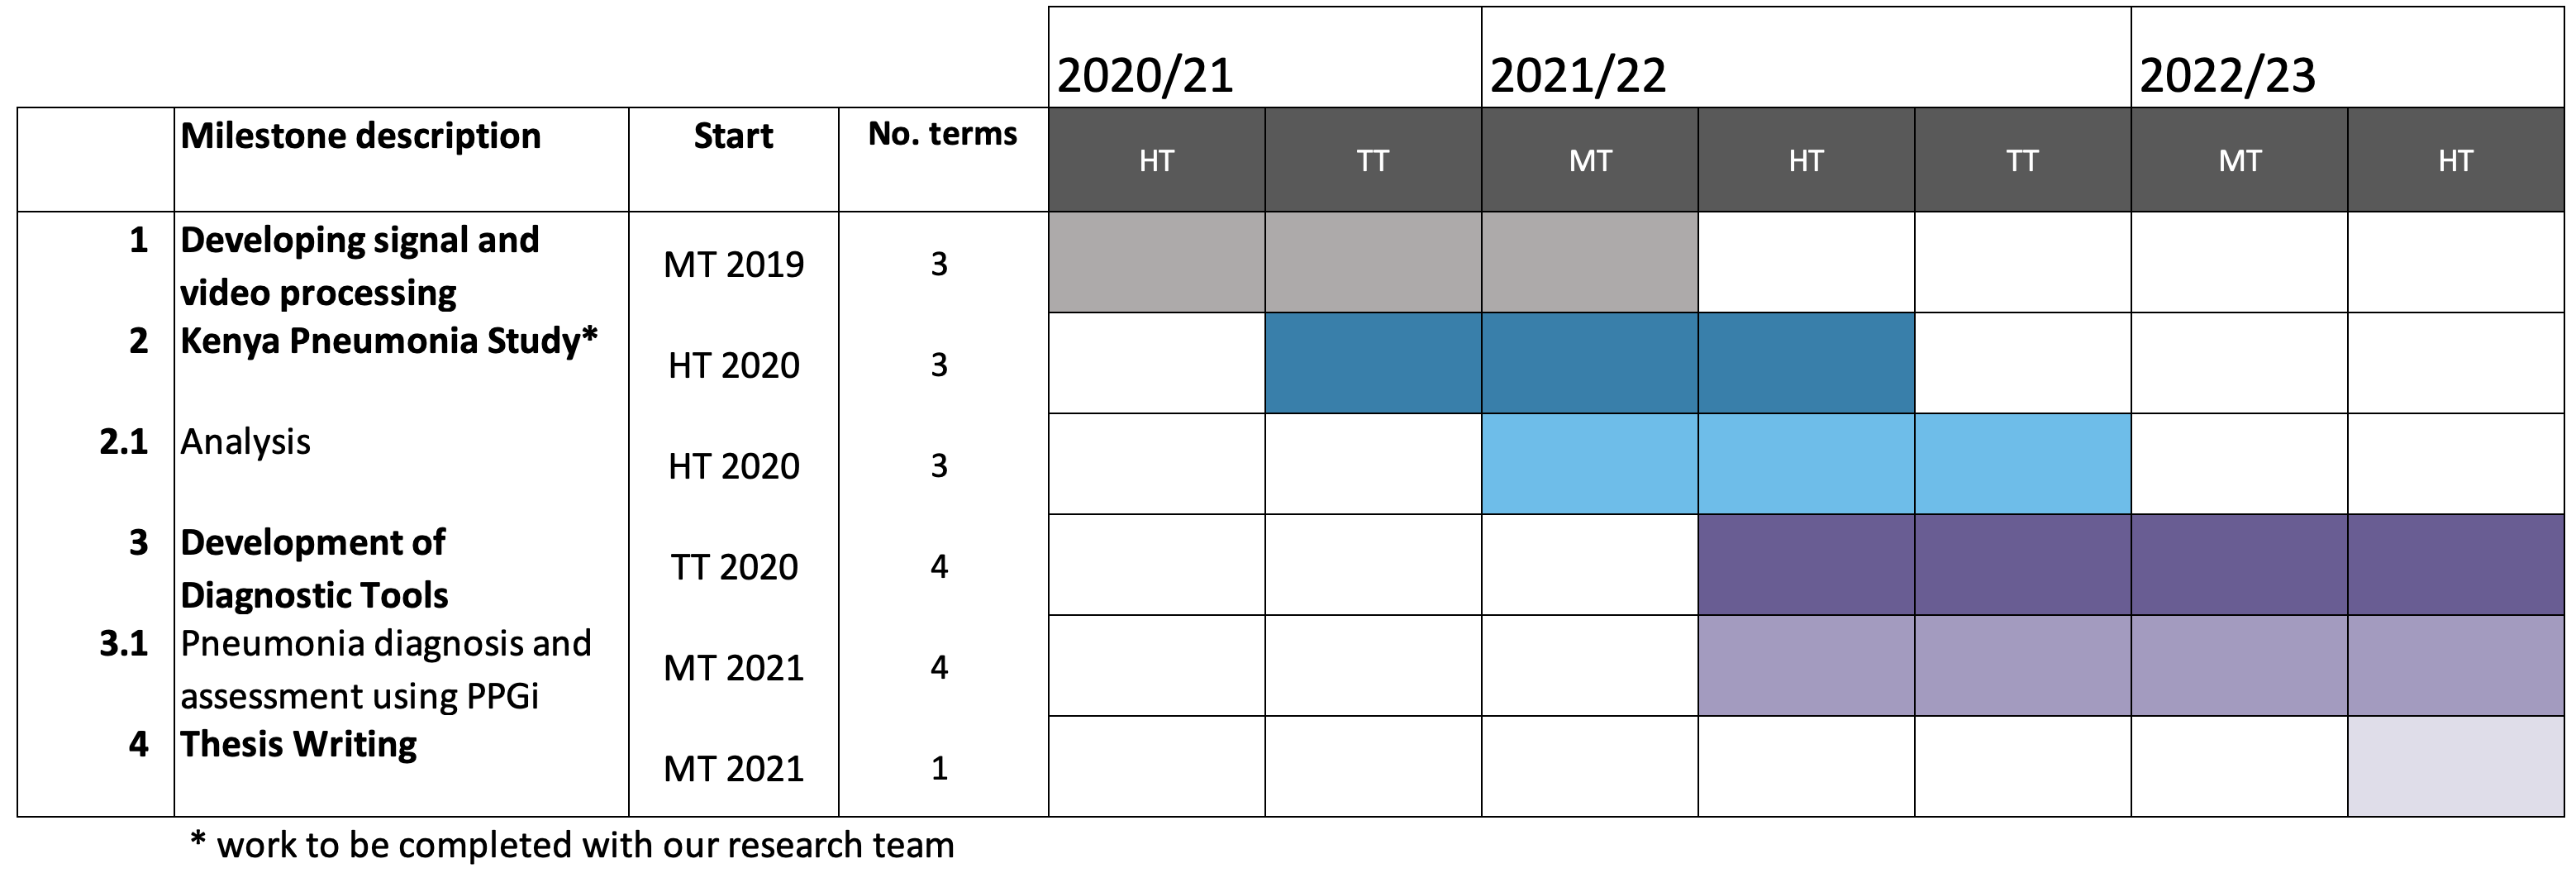
\includegraphics[width = 14 cm]{nicu_Gantt_Chart.png}
 \caption[Gantt Chart for Dphil project timeline.]{Gant Chart for Dphil project timeline.}
     \label{gantchart}
\end{figure}